\chapter{Conclusion}
Dans ce mémoire, j'ai exploré les origines de l'art de la \textit{demoscene} et examiné les techniques essentielles pour une performance de \textit{livecoding} de \textit{shaders} réussie. Par la suite, j'ai centré mon analyse sur l'interaction authentique entre la musique et le visuel, dans l'espoir de contribuer modestement à l'évolution de la \textit{demoscene}.

\paragraph*{Mes expérimentations}
Au cours de mes explorations, j'ai réalisé quelques expérimentations disponibles sur Vimeo. Bien qu'en l'état peu ambitieuses, elles servent de preuve de concept\footnote{Un \textit{proof of concept} (POC), traduit littéralement en français par «~preuve de concept~», est une démonstration ou un prototype qui vise à prouver la faisabilité ou la viabilité d'une idée, d'un concept ou d'une méthode.} : si j'ai réussi à modifier le rayon d'un cercle uniquement avec la vélocité de la note jouée, cela démontre la possibilité d'agir sur n'importe quelle variable définie dans le code GLSL (voir \ref{experim00} et \ref{experim01} \href{https://vimeo.com/user167850166}{sur ma page Vimeo}). 

\begin{figure}[h]
  \begin{minipage}[b]{0.45\linewidth}
    \centering
    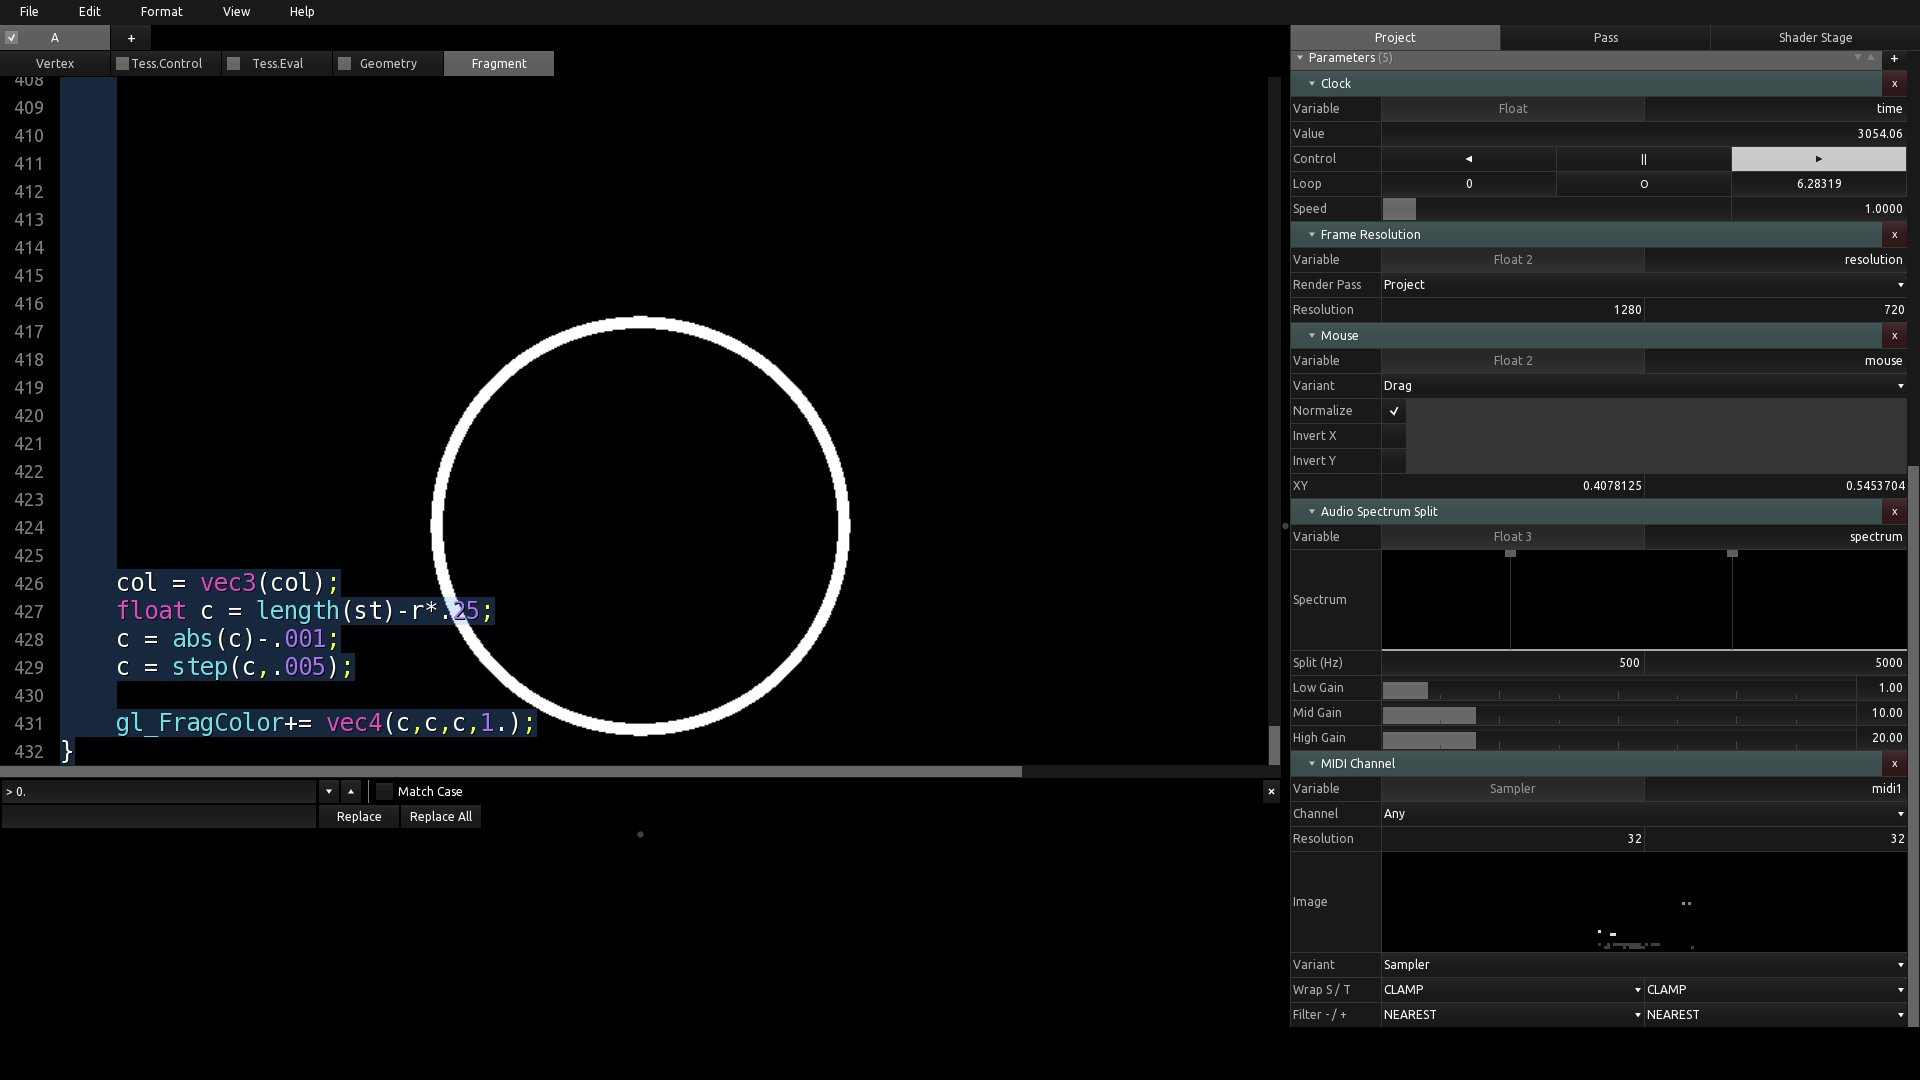
\includegraphics[width=\linewidth]{images/experiments/intensifs/experim00.png}
    \caption{\textit{Live} avec un flux MIDI composé en C}
    \label{experim00}
  \end{minipage}
  \hspace{0.1\linewidth} % Espace horizontal pour la gouttière
  \begin{minipage}[b]{0.45\linewidth}
    \centering
    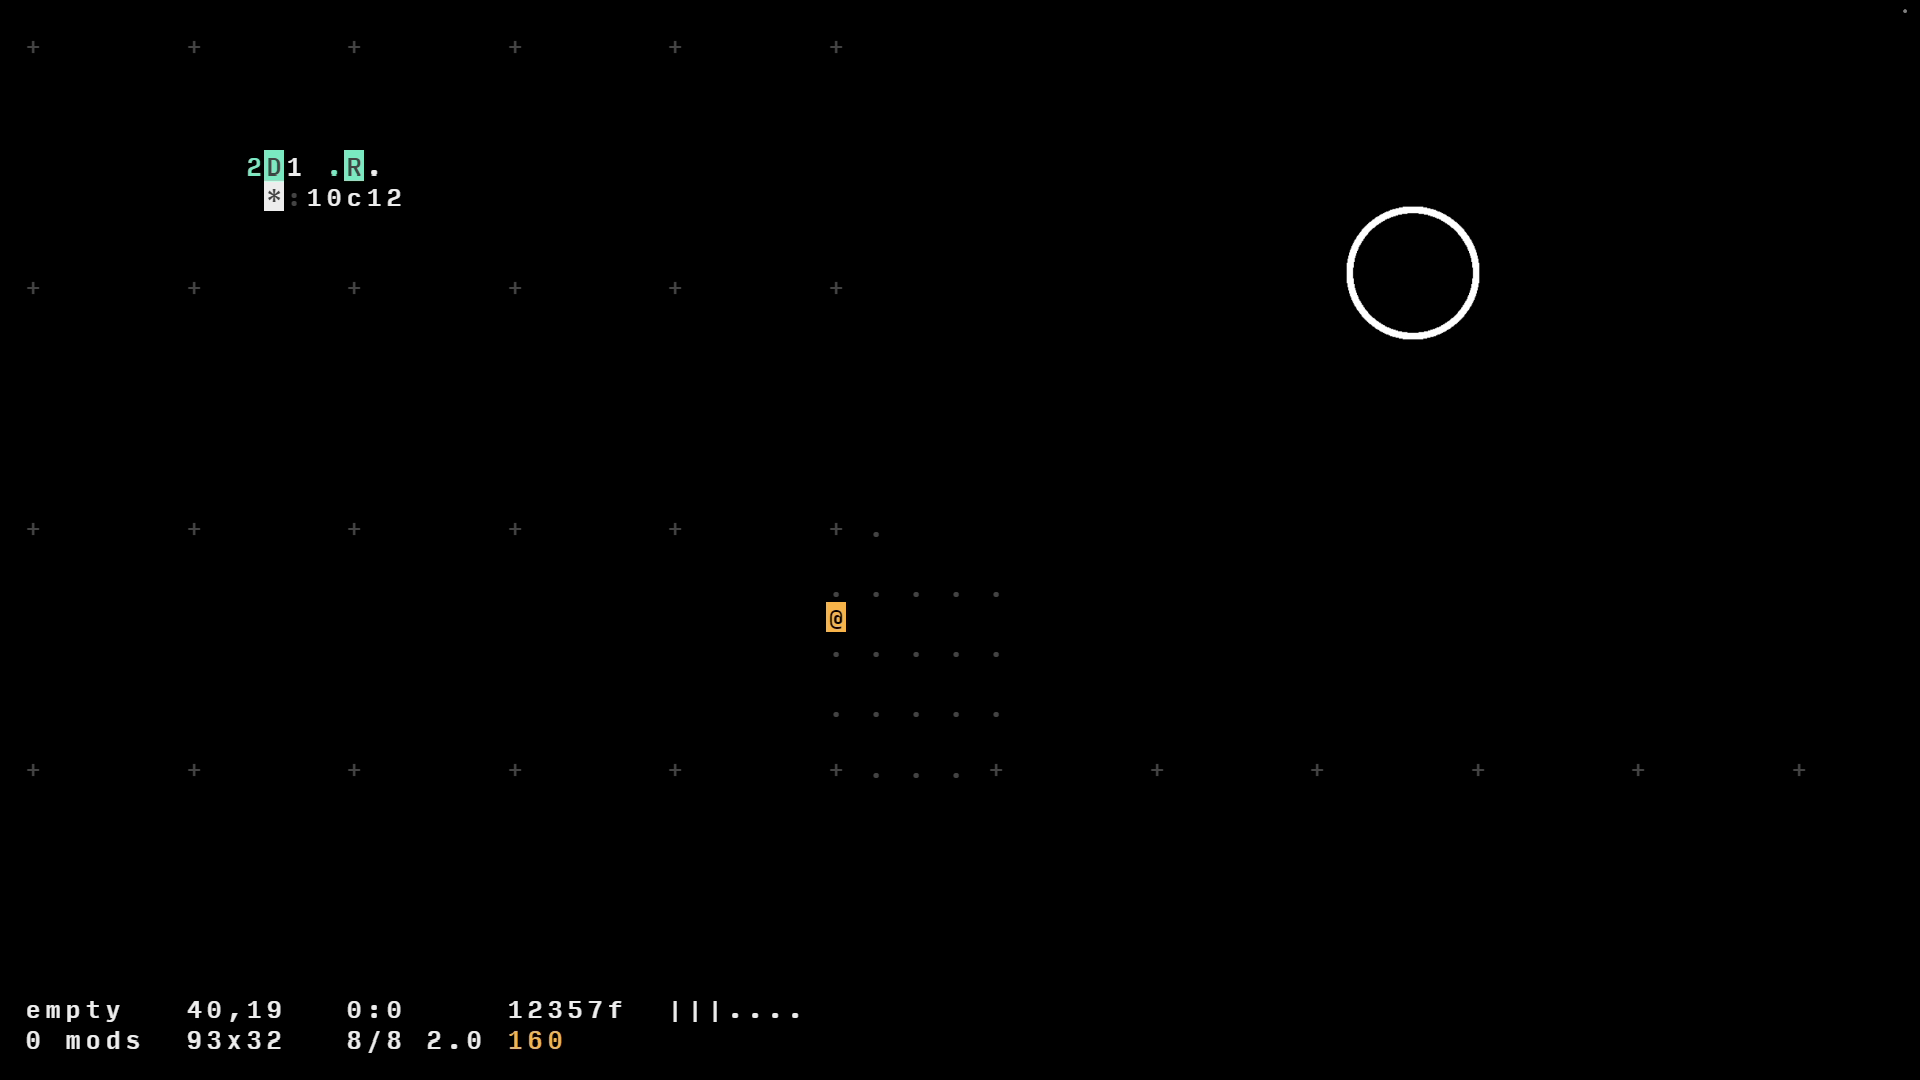
\includegraphics[width=\linewidth]{images/experiments/intensifs/experim01.png}
    \caption{\textit{Live} avec une note aléatoire}
    \label{experim01}
  \end{minipage}
  %\caption{Animation de visuels avec Orca 2}
\end{figure}



Maintenant que j'ai confirmé que les mécanismes interactifs nécessaires sont déjà établis et fonctionnels, je suis prêt à explorer ce nouveau \textit{pipeline} qui répond parfaitement à mes attentes. À chaque itération, j'améliore le flux de travail en factorisant le code, en ajoutant des fonctionnalités, en peaufinant l'animation, etc. (voir \ref{experim03} et \ref{experim02})

\begin{figure}[h]
  \begin{minipage}[b]{0.45\linewidth}
    \centering
    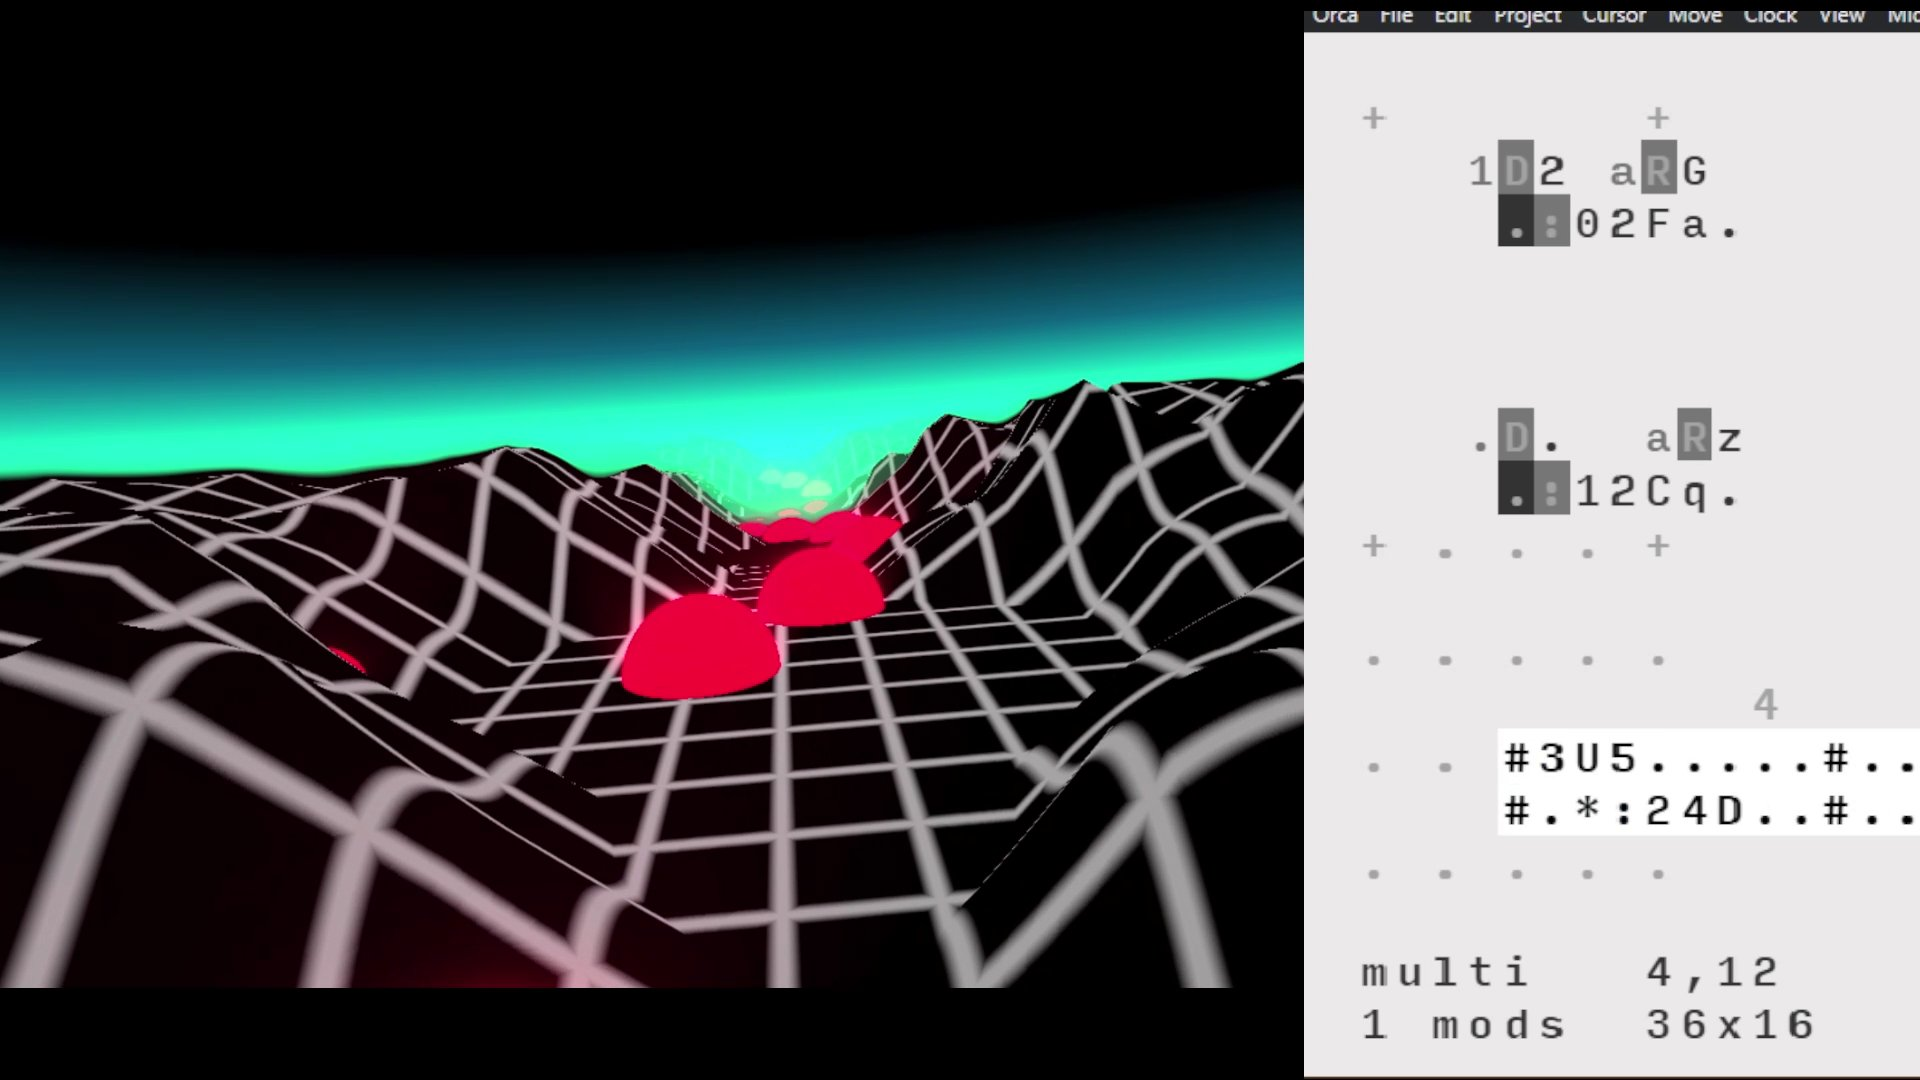
\includegraphics[width=\linewidth]{images/experiments/experim03.png}
    \caption{Animation d'un \textit{shader}}
    \label{experim03}
  \end{minipage}
  \hspace{0.1\linewidth} % Espace horizontal pour la gouttière
  \begin{minipage}[b]{0.45\linewidth}
    \centering
    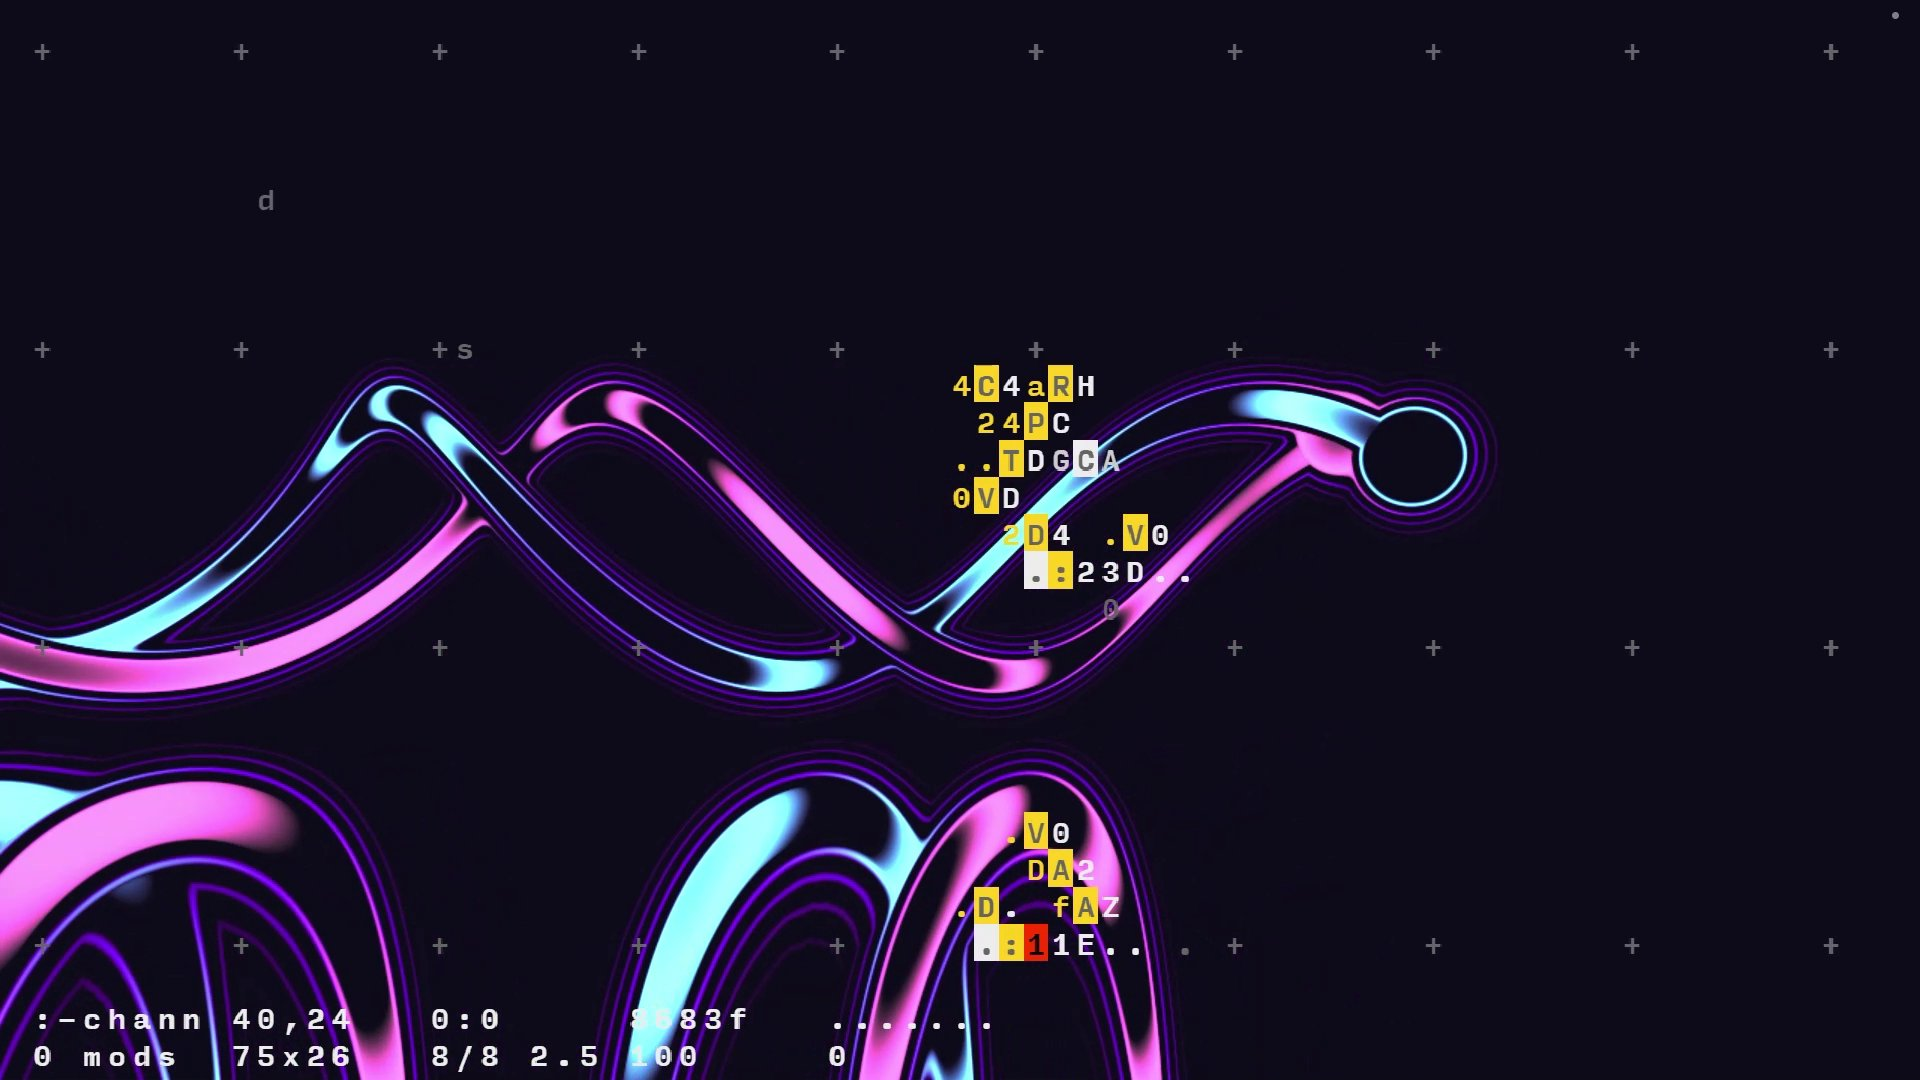
\includegraphics[width=\linewidth]{images/experiments/experim02.png}
    \caption{\textit{Hack} pour la transparence d'Orca}
    \label{experim02}
  \end{minipage}
  %\caption{Animation de visuels avec Orca 2}
\end{figure}




\paragraph*{Journée d'étude sur le \textit{live coding}}

Un récent événement qui a profondément marqué mon expérience était la «~journée d'étude sur le live coding~», orchestrée par Raphaël Forment, Rémi Georges et Agathe Herrou à la Maison des Sciences de l'Homme à La Plaine St-Denis (voir \ref{jlc00}). Cette journée comprenait une série de conférences suivies de performances sonores et visuelles. C'est lors de cet événement que j'ai vraiment pris conscience que le \textit{livecoding} était un véritable domaine de recherche et de création, réunissant des artistes, des chercheurs et des passionnés aux parcours différents autour d’un geste commun : celui de manipuler du code source « à la volée » dans un but d'expression artistique et de création. Une présentation qui a captivé mon attention est celle de Vincent Rioux : \textit{Redécouvrir le live-coding en LISP, i-a-d-d-la-joie ! – Utiliser Lisp et Supercollider avec une intelligence simple}. Son travail met en avant la création d'un lien entre la musique et les arts visuels, notamment entre les Beaux-Arts de Paris et l'IRCAM (Institut de Recherche et de Coordination Acoustique/Musique). Je prévois d'approfondir ses travaux, car les sujets qu'il aborde semblent étroitement liés aux miens.

\begin{figure}[h]
    \centering
    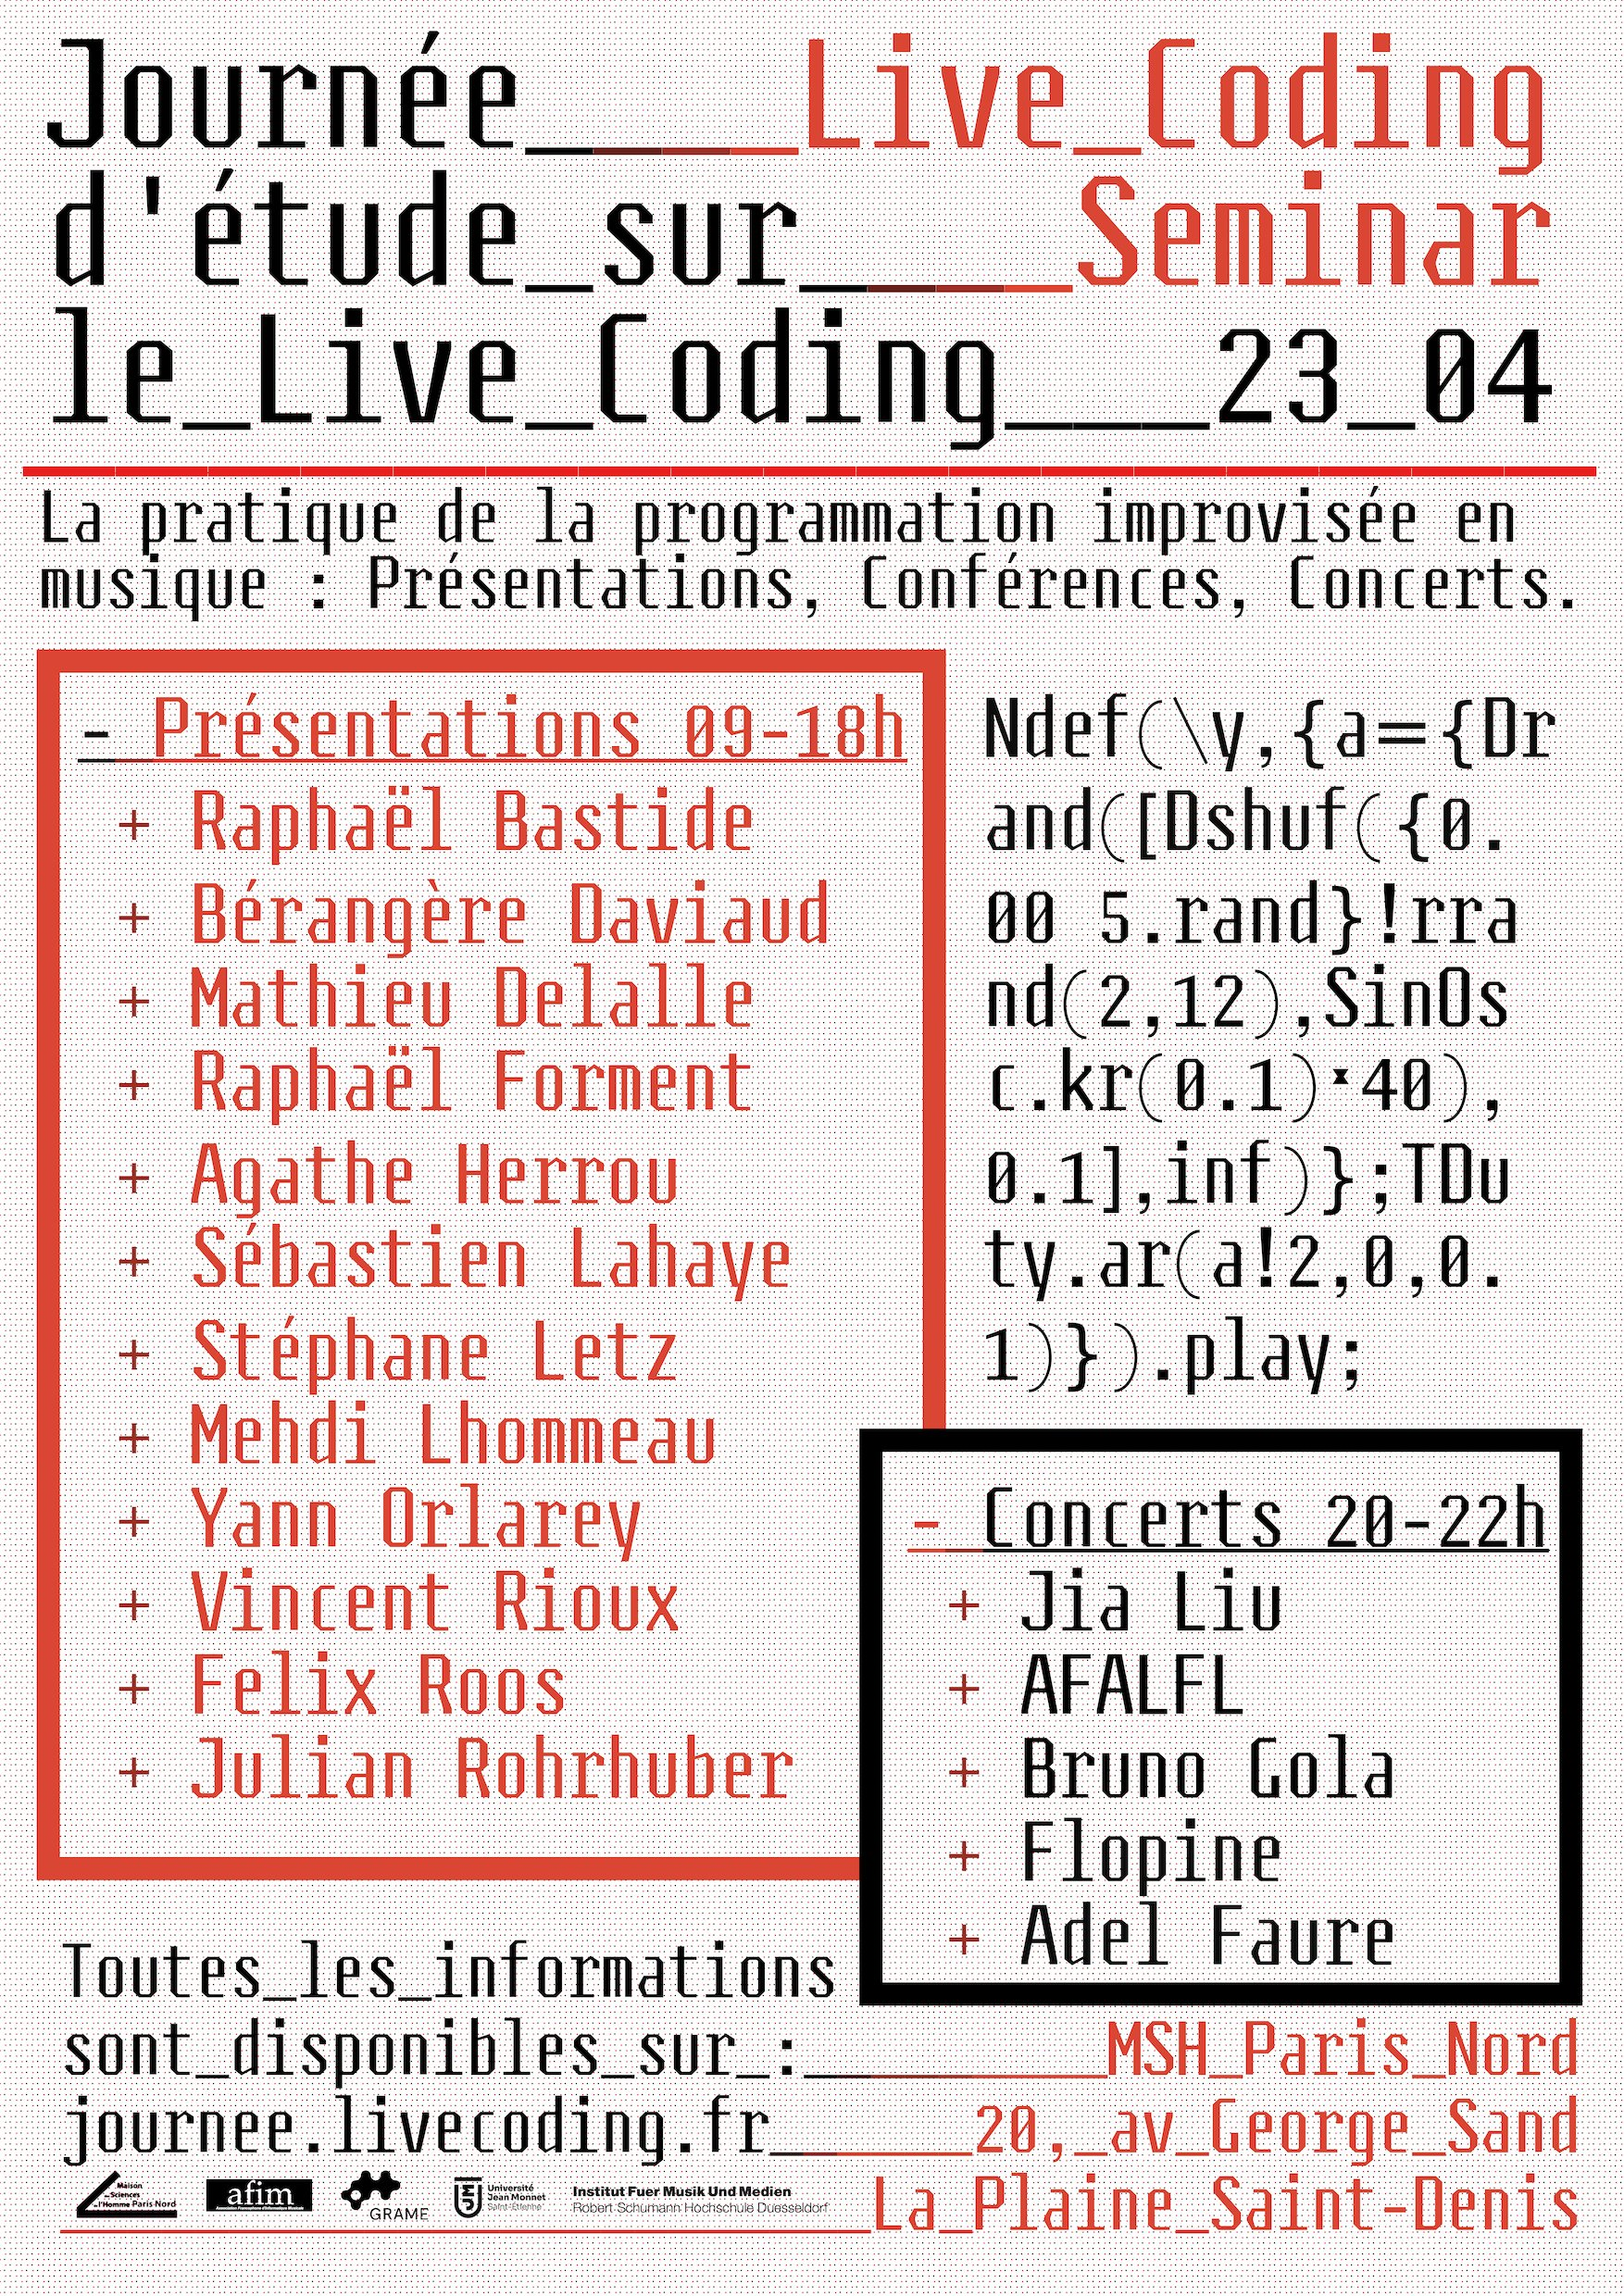
\includegraphics[width=6cm]{images/jlc_affiche.png}
    \caption{Affiche de la journée d’étude sur le \textit{livecoding}}
    \label{jlc00}
\end{figure}



\paragraph*{Vers un mélange des arts et la démocratisation de la \textit{demoscene}}
Grâce aux rencontres que j'ai pu faire cette année lors des événements organisés par le Cookie Collective, j'ai eu l'opportunité d'explorer de nouvelles perspectives. En particulier, ma brève rencontre avec Alexandre et Sharlaine, les organisateurs du Playground (voir \ref{peanut}), un événement dédié au \textit{creative coding} à Bordeaux, m'a profondément inspiré (leur site est consultable \href{https://plgrnd.cc/}{ici}). Leur approche originale renforce mon désir de rendre la \textit{demoscene} plus accessible en mettant l'accent sur la diffusion d'une éducation technique capable de sensibiliser et d'impliquer un public plus large. De plus, leur collaboration en tant que duo, « La Peanut », qui combine le \textit{livecoding}, le théâtre et la poésie, reflète également mes aspirations à faire progresser mes recherches et mes créations numériques vers un «~mélange des arts~». Ces arts pourraient inclure des récitations de texte (narratives ou non), l'intégration d'instruments acoustiques ou encore la manipulation de vidéos en direct.


\begin{figure}[h]
  \begin{minipage}[b]{0.45\linewidth}
    \centering
    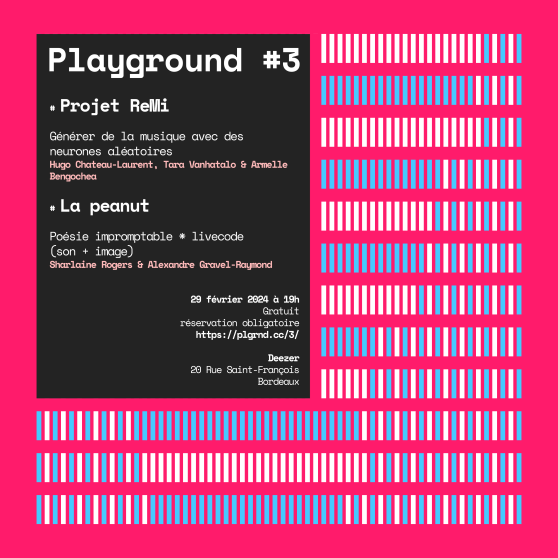
\includegraphics[width=.8\linewidth]{images/conclusion/peanut00.png}
  \end{minipage}
  \hspace{0.1\linewidth} % Espace horizontal pour la gouttière
  \begin{minipage}[b]{0.45\linewidth}
    \centering
    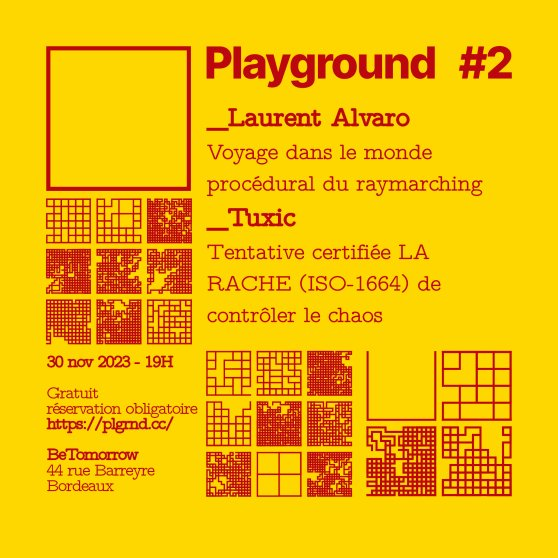
\includegraphics[width=.8\linewidth]{images/conclusion/peanut01.png}
  \end{minipage}
  \caption{Programme du Playground organisé par Alexandre}
  \label{peanut}
  %\caption{Animation de visuels avec Orca 2}
\end{figure}

\paragraph*{Vers une communication réseau}

Jusqu'à présent, mes expérimentations techniques ont été réalisées sur une seule machine. Cependant, comme l'indique le titre de mon mémoire, « \textit{Vers une interaction authentique entre livecoders} », cela illustre également mon désir initial d'impliquer plusieurs \textit{livecoders} au cours d'une même performance. En pratique, un \textit{livecoder} serait responsable de la création musicale sur Orca et enverrait les informations MIDI via le réseau à une autre machine contrôlée par un \textit{livecoder} de \textit{shaders}. Cet objectif constituait le cœur de mon intensif en M2. Malheureusement, notre groupe a dû faire face à de nombreuses complications, à la fois matérielles et logistiques, qui nous ont empêché d'atteindre cet objectif dans les délais impartis. Cependant, avec le recul, j'ai découvert l'existence de solutions déjà disponibles qui auraient pu nous faciliter la réalisation. Parmi les solutions envisagées, je compte explorer Troop et Flok, des logiciels permettant à plusieurs utilisateurs de pratiquer le \textit{livecoding} musical sur un serveur commun. 
Dans mes futures recherches, je m'efforcerai de trouver une solution équivalente mais orientée vers l'intégration collaborative du visuel et du sonore.

\newpage
\begin{figure}[h]
    \centering
    
\includegraphics[width=6cm]{images/conclusion/stribe.png}
    \caption{Goodbye!}
    \label{stribe00}
\end{figure}



